\section{Background}

\begin{frame}{}
  \begin{center}
    \Large{Why is this not about ANNS anymore?}
  \end{center}
\end{frame}

\begin{frame}{Problem Statement}
  \begin{definition}[Random Sampling without Replacement]
    Given a data set \(X\), we want to uniformly pick \(k\) elements from \(X\) such
    that none of them repeat.
  \end{definition}
\end{frame}

\begin{frame}{Baseline}
  The baseline solution: \textit{Priority Sampling}
  \begin{algorithm}[H]
  \caption{Priority Sampling}
  \begin{algorithmic}
    \State{Fill in later}
  \end{algorithmic}
  \end{algorithm}
\end{frame}

\begin{frame}{Baseline}
  \begin{algorithm}[H]
  \caption{Parallel Priority Sampling}
  \begin{algorithmic}
    \State{Fill in later}
  \end{algorithmic}
  \end{algorithm}
\end{frame}

\begin{frame}{A different approach: Permutation}
  \begin{itemize}
    \item Shuffle then take first \(k\).
    \item Shuffling process doesn't have to \textit{"complete"}.
  \end{itemize}
\end{frame}

\begin{frame}{Permutation via Knuth Shuffle}
  \begin{algorithm}[H]
  \caption{Fisher-Yates}
  \begin{algorithmic}
    \State{Fill in later}
  \end{algorithmic}
  \end{algorithm}
\end{frame}

\begin{frame}{Permutation via Knuth Shuffle}
  \begin{center}
    \Large{Small issue: It's very sequential!}
  \end{center}
\end{frame}

\begin{frame}{Parallel Knuth Shuffle}
  According to Shun et al. \cite{julian-parperm}, you can run Knuth Shuffle in
  parallel.

  \begin{figure}
    \begin{center}
      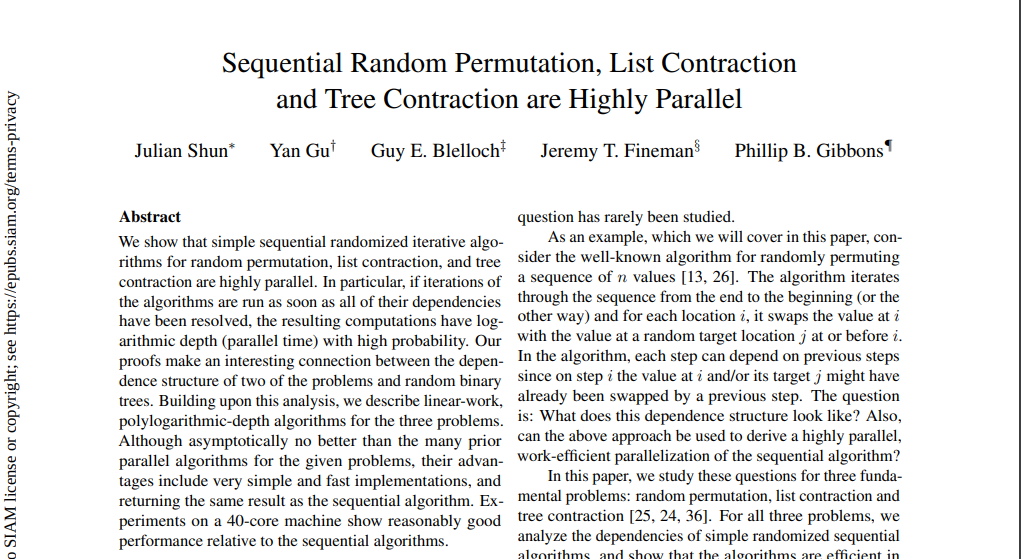
\includegraphics[width=0.60\textwidth]{julian-paper}
    \end{center}
    \caption{Shun et al. \cite{julian-parperm}}
  \end{figure}
\end{frame}

\begin{frame}{Parallel Knuth Shuffle}
  \begin{center}
    \Large{ Main result: Knuth Shuffle can be run with \(\Theta(n)\) work and
    \(O(\log n)\) span. }
  \end{center}
\end{frame}

\begin{frame}{Deterministic Reservation}
  A framework by Blelloch et al. \cite{blelloch-detreserve} for developing
  parallel algorithms.
  \begin{itemize}
    \item Splits iteration into 2 phases: Reservation and Committing
    % \item Reserve decides what should be processed.
    % \item Commit carries out the processing.
    \item Primitive: \textsc{WriteMax(\(l, x\))} 
  \end{itemize}
\end{frame}
